\chapter{Interface utilisateur\\ (Adrian)}

Cette partie n'était pas nécessaire pour la première soutenance, mais une petite
interface simple et fonctionnelle permet de tester rapidement nos différentes
implémentations. La bibliothèque SDL est assez limitée en termes d'interface
utilisateur, c'est pourquoi nous avons utilisé la bibliothèque GTK+ pour cette
tâche.

Cependant, écrire une interface en dur dans le code est un processus fastidieux
et source d'erreurs. GTK+ contourne ce problème en permettant de charger une
description XML de l'interface. L'outil de design d'interface utilisateur
\textit{Glade} nous donne la possibilité de créer cette interface en quelques
minutes et de l'exporter en format XML lisible par GTK+.

\newpage

L'interface est alors composée de quelques boutons sur le menu gauche, ainsi que
de l'image actuellement chargée en mémoire au centre de l'écran :

\begin{figure}[H]
    \centering
    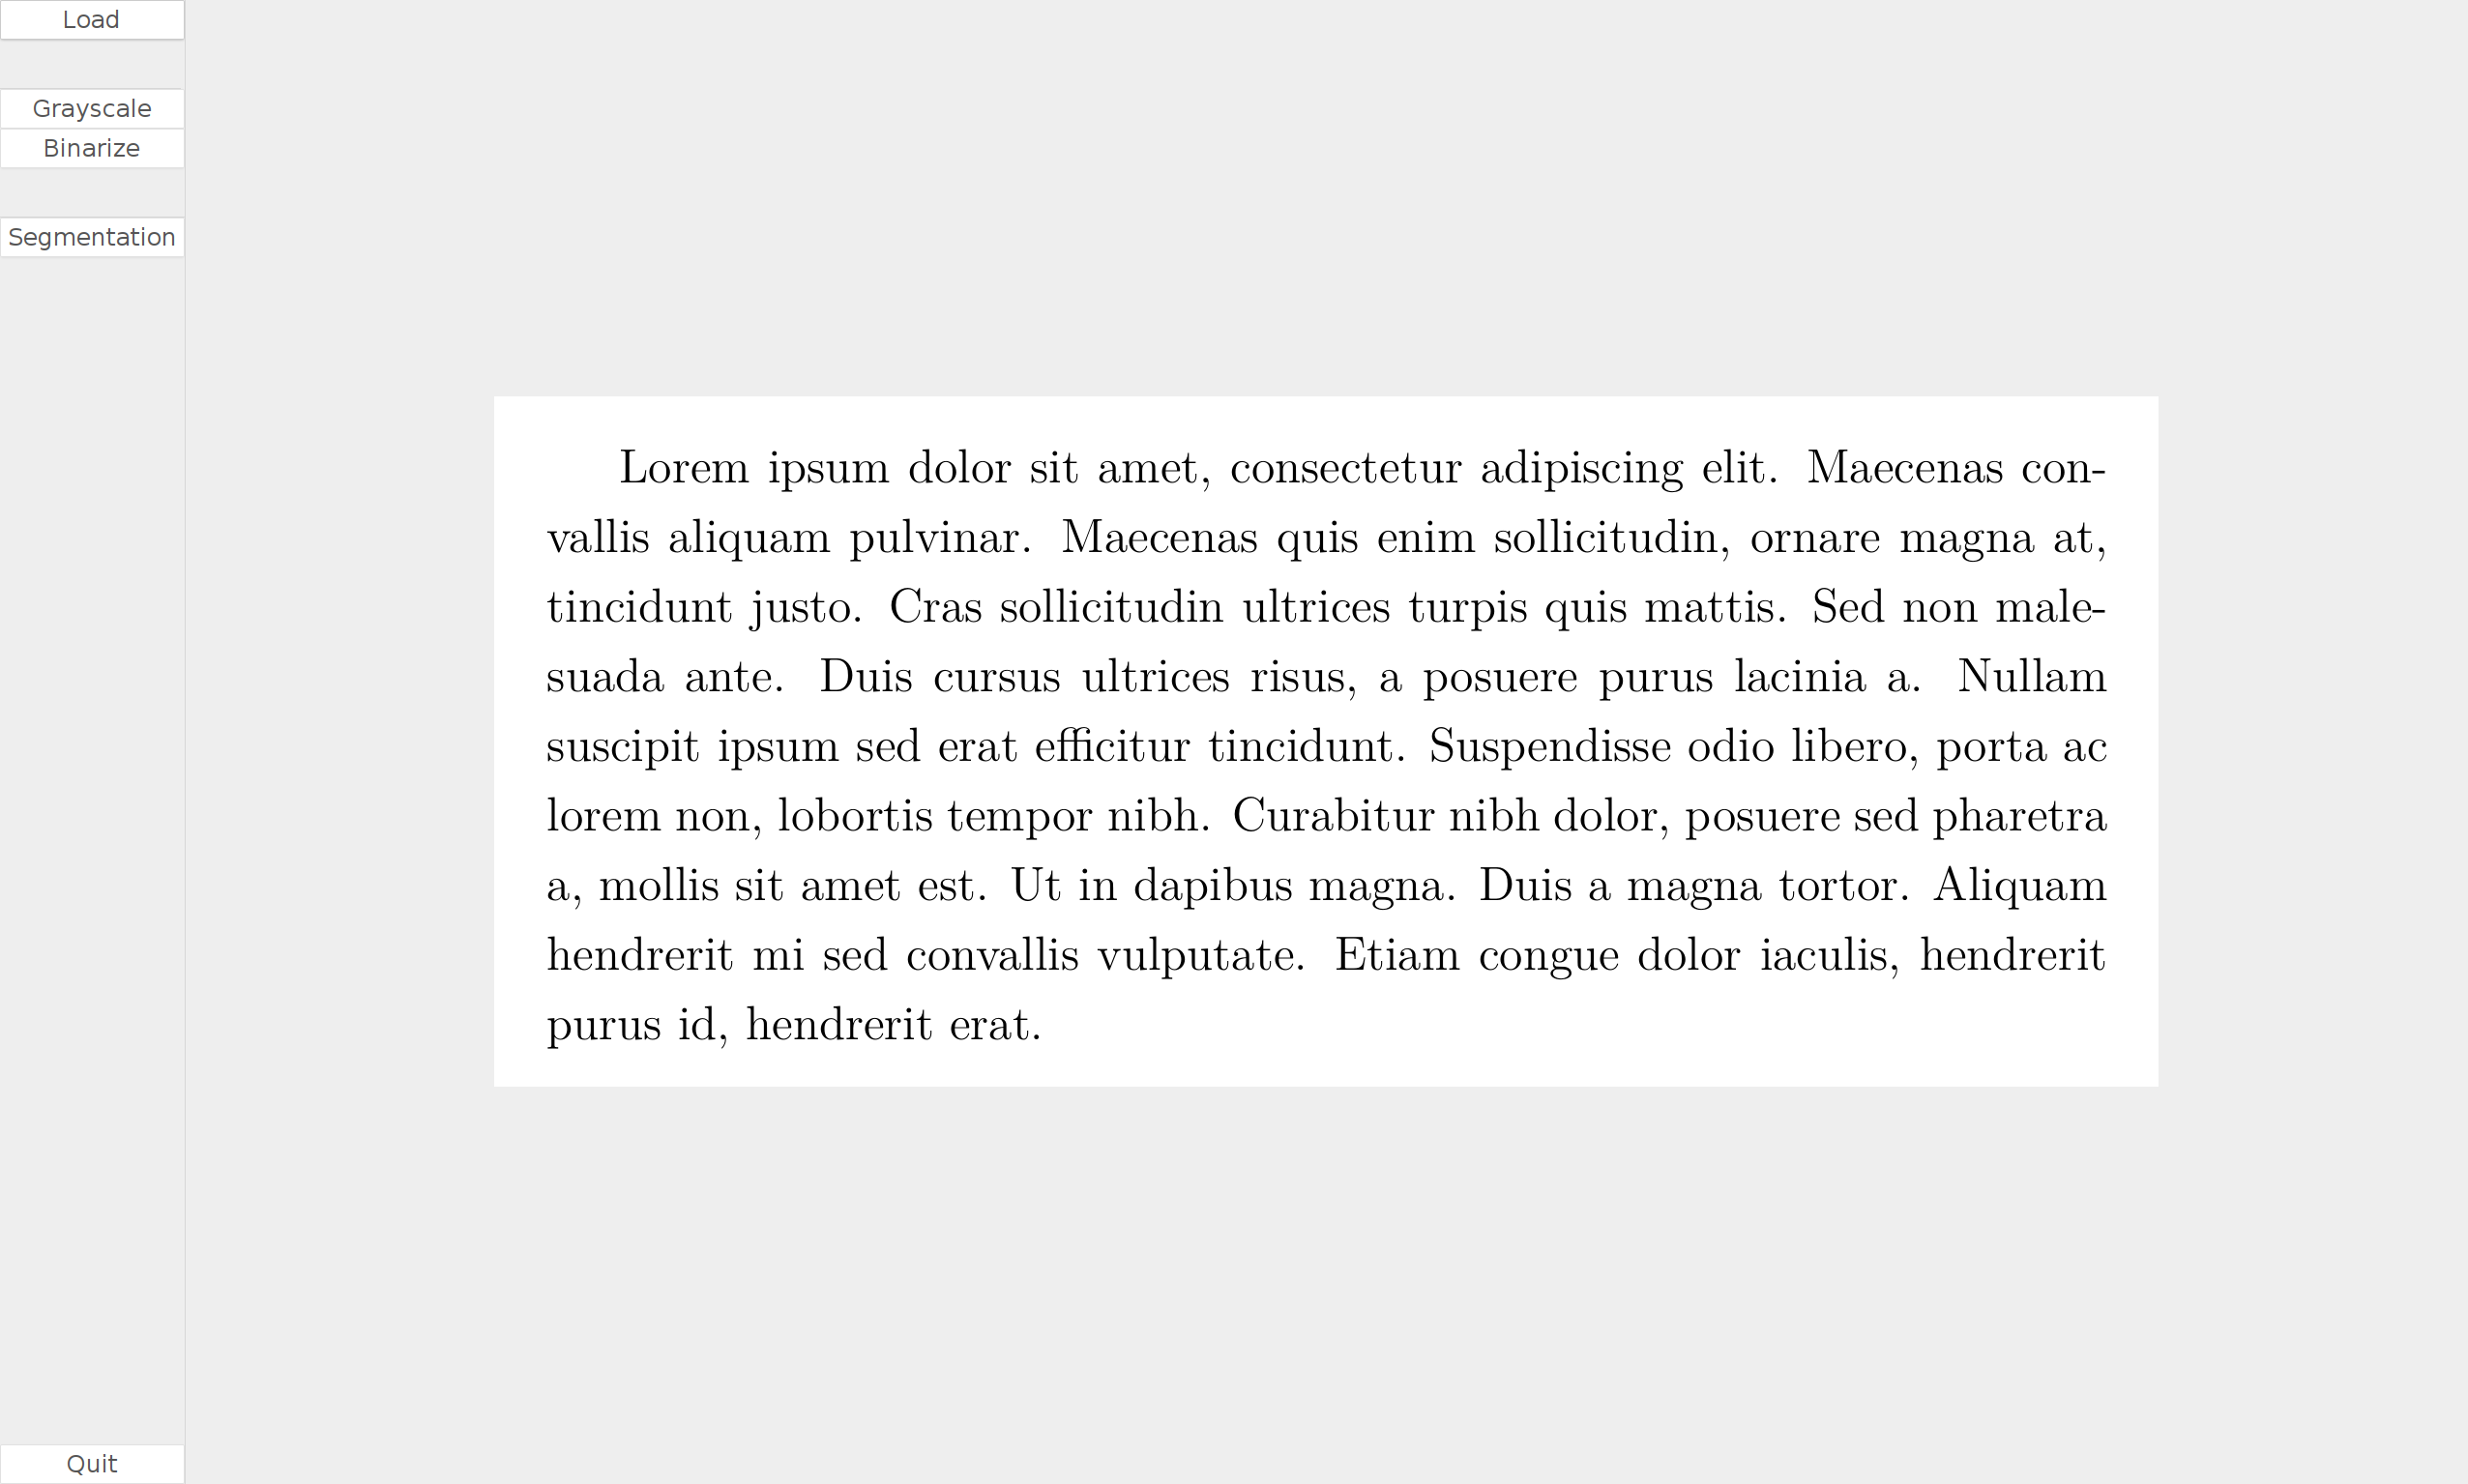
\includegraphics[width=0.9\textwidth]{interface}
    \caption{Interface utilisateur}
\end{figure}
